\documentclass[8pt]{beamer}

\usepackage{bm}% bold math
\usepackage{color}
\usepackage{tcolorbox}
\usepackage{lipsum}
\usepackage{tikz}
\usepackage[backend=biber]{biblatex}

\usepackage{color}
\setlength{\tabcolsep}{1.3pt}
\usepackage{bm}
\usepackage{amsmath}
\usepackage{amssymb}
\usepackage{mathtools}
\usepackage{mathrsfs}
\usepackage[T1]{fontenc}
%\usepackage{stfloats}
\usepackage{diagbox}
\usepackage{here}
%\usepackage[dvipsnames]{xcolor}
\usepackage{multirow}
\usepackage{ctable} % for \specialrule command
\usepackage{array,booktabs}
\newcolumntype{M}[1]{>{\centering\arraybackslash}m{#1}}
\usepackage{subcaption}
\usepackage{float}
\usepackage{unicode-math}

\restylefloat{table}
\numberwithin{equation}{section}

\usepackage{epstopdf}
\epstopdfDeclareGraphicsRule{.tga}{png}{.png}{%
  convert #1 \OutputFile
}
\AppendGraphicsExtensions{.tga}
\newcommand{\etal}{{\textit{et al.}}}

\DeclareMathOperator*{\argmax}{arg\,max}
\DeclareMathOperator*{\argmin}{arg\,min}


%\usetheme{Warsaw}
%\usecolortheme{seahorse}
\definecolor{myblue1}{RGB}{35,119,189}
\definecolor{myblue2}{RGB}{52,74,154}
\setbeamercolor*{structure}{fg=myblue2}

%\setbeamercolor{frametitle}{fg=myblue2,bg=myblue2!10}

\setbeamertemplate{frametitle}{\color{myblue2}\bfseries\insertframetitle\par\vskip-6pt\hrulefill}
\addtobeamertemplate{navigation symbols}{}{%
    \usebeamerfont{footline}%
    \usebeamercolor[fg]{footline}%
    \hspace{1em}%
    \insertframenumber/\inserttotalframenumber
}
\setbeamerfont{footline}{series=\bfseries}

%\titlegraphic{
\includegraphics[scale=0.3]{Figures/Freiburg.jpg}}
\logo{
\includegraphics[scale=0.12]{Figures/20221107-UFR-logo-blue-rgb-344A9A.pdf} \hspace{4.5cm} 
\includegraphics[scale=0.45]{Figures/Freiburg.jpg}} 
\newcommand{\nologo}{\setbeamertemplate{logo}{}}
\title[]{Bayesian Optimization}
%\subtitle{MASTER THESIS}
\vspace{3mm}
\author[Polina Gaindrik]{Polina Gaindrik}

\institute{University of Freiburg\\
Freiburg Center for Data Analysis and Modeling (FDM) \\ Spatial Systems Biology Group}
\date{03.06.2025}


\begin{document}
\addtocounter{framenumber}{-1}  
\frame {
	\titlepage

}


{\nologo \frame{	
	\frametitle{Bayesian Optimization}

Problem formulation:
\begin{equation*}
    \max_{x \in A} f(x), \hspace{3mm} x \in R^d, \hspace{3mm} d \leq 20
\end{equation*}

\vspace{3mm}
\begin{itemize}
    \item $A$: hyper-rectangle or $d$-dimensional simplex
    \item $f$ is a continuous objective function
    \item $f$ is a "black-box": structure of the function is not known
\end{itemize}

\vspace{3mm}
Advantages of the Bayesian Optimization:

\begin{itemize}
    \item No 1st- or 2nd-order derivatives of the $f(x)$ needed
    \item Number of evaluation of the $f(x)$ is limited (hundreds)
    \item Global Optimization
\end{itemize}


}}

{\nologo \frame{	
	\frametitle{Bayesian Optimization: Workflow}
    \begin{columns}
        \column{0.47\linewidth}
            \begin{enumerate}
                \item Set a prior distribution of $f(x)$ for Gaussian Processes (GP) regression

                \item For initial sampling $D_0$
                update the posterior distribution of the objective $f$
                \vspace{2mm}
                \item
                \begin{itemize}
                    \item Choose the new $n+1$ sampling point $\tilde x$ using acquisition function 
            
                    \item Calculate function $f(\tilde x)$

                    \item Update posterior distribution of $f(x)$
                \end{itemize}

                \vspace{2mm}
                \item Repeat point 3 until the number of sampling points $n=N$
            \end{enumerate}

    \column{0.55\linewidth}
        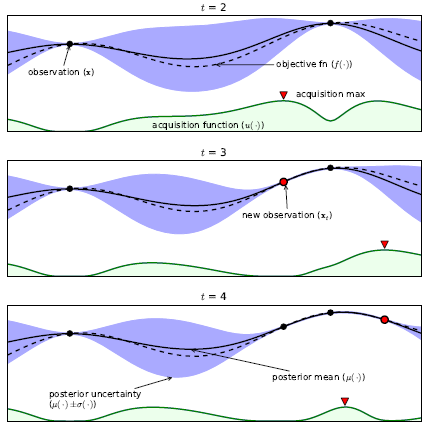
\includegraphics[scale=0.5]{Figures/BayesOpt_scheme.PNG} 
    \end{columns}

}}

{\nologo \frame{	
	\frametitle{Gaussian Process (GP) Regression}

    For an initial input $D_0 = x_{1:n} = (x_1,..., x_n)$
    the resulting prior distribution:
    \begin{equation*}
        f(x_{1:n}) \propto N(\mathbf{\mu}_0(\mathbf{x}_{1:n}), \Sigma_0^2(\mathbf{x}_{1:n}))
    \end{equation*}

    \vspace{2mm}
    Here mean and covariance matrix function:
   \begin{equation*}
       \mathbf{\mu}_0(\mathbf{x}_{1:n}) = (\mathbf{\mu}_0(\tilde x_1), ..., \mathbf{\mu}_0(x_n))
   \end{equation*}

    \begin{equation*}
       \Sigma_0 (\mathbf{x}_{1:n}, \mathbf{x}_{1:n}) = \begin{pmatrix}
           \Sigma_0 (x_1, x_1)& ...&  \Sigma_0 (x_1, x_n)\\
           \vdots &  & \vdots\\
           \Sigma_0 (x_n, x_1)& ...&  \Sigma_0 (x_n, x_n)\\
       \end{pmatrix}
    \end{equation*}

}}


{\nologo \frame{	
	\frametitle{Gaussian Process Regression}

    Given previous iteration step head $n$ points $\mathbf{x}_{1:n} = (x_1, ..., x_n)$
    adding new sampling point $\tilde x$ give conditional distribution of $f(x)$:

    \begin{equation*}
        f(\tilde x)|f(\mathbf{x}_{1:n}) \propto N(\mu_n(\tilde x), \sigma_n^2(\tilde x))
    \end{equation*}

    Posterior mean:
    \begin{equation*}
        \mu_n (\tilde x) = \Sigma_0 (\tilde x, \mathbf{x}_{1:n}) \Sigma_0 (x_{1:n}, \mathbf{x}_{1:n})^{-1} (f(\mathbf{x}_{1:n})-\mu_0 (\mathbf{x}_{1:n})) + \mu_0 (\tilde x)
    \end{equation*}

    Posterior variance:
    \begin{equation*}
        \sigma^2_n (\tilde x) = \Sigma_0 (\tilde x, \tilde x) - \Sigma_0 (\tilde x, \mathbf{x}_{1:n}) \Sigma_0 (\mathbf{x}_{1:n}, \mathbf{x}_{1:n})^{-1} \Sigma_0 (\mathbf{x}_{1:n}, \tilde x)
    \end{equation*}


}}

{\nologo \frame{	
	\frametitle{Gaussian Process Regression: choosing prior}
    Mean function:
    \begin{itemize}
        \item Constant value $\mu_0 = \mu$
        \item $\mu_0 = \mu + \sum_{i=1}^p \beta_i \psi_i (x)$\\
        $\psi_i$: parametric function, often low-order polynomial
    \end{itemize}

    \vspace{3mm}
    Kernel function:
    \begin{itemize}
        \item If $|x-x'|<|x-x''|$ then $\Sigma_0(x, x')<\Sigma_0(x, x')$
        \item Positive semi-definite function

        \item Power exponential (Gaussian) kernel:
        \begin{equation*}
            \Sigma_0(x, x') = \alpha_0 \exp (-\sum_{i=1}^d \alpha_i (x_i-x_i')^2)
        \end{equation*}
        \item Matern kernel
    \end{itemize}

    \vspace{3mm}
    Optimizing hyperparameters $(\alpha, \mu, \beta)$
    \begin{itemize}
        \item Maximum likelihood estimation
        \item Integrating over hyperparametrs distribution $P(\alpha, \mu, \beta)$
    \end{itemize}
    

}}


{\nologo \frame{	
	\frametitle{Acquisition function}

    \textbf{Expected Improvement (EI)} of the evaluation at the point $\tilde x$:
    \begin{equation*}
        EI_n (\tilde x) = E_n [\max(f(\tilde x)-f^*_n, 0)]
    \end{equation*}
    $E_n$: the expectation taken under the posterior distribution calculated n the previous step with mean $\mu_n(\tilde x)$ and variance $\sigma^2_n (\tilde x)$\\
    $f^*_n = \max f({\mathbf{x}_{1:n}})$

    \vspace{3mm}
    Expected improvement algorithm:

    \begin{equation*}
        x_{n+1} = \argmax EI_n (\tilde x)
    \end{equation*}

    \begin{itemize}
        \item EI is inexpensive to evaluate
        \item Can be solved with 1st-, 2nd-order optimization methods (e.g., quasi-Newton method L-BFGS-B)
        \item Balances between points with high expected quality, large $f(\tilde x)-f^*_n$, and high uncertainty $\sigma_n(\tilde x)$
    \end{itemize}

}}


{\nologo \frame{	
	\frametitle{Acquisition function}
      \textbf{Knowledge Gradient (KG)}:
      \begin{equation*}
          KG_n(\tilde x) = E_n [\mu^*_{n+1} - \mu^*_{n}|x_{n+1}=\tilde x]
      \end{equation*}
      where $\mu^*_{n} = \max_{x} \mu_n (x)$

    \vspace{3mm}
      \begin{itemize}
          \item More suitable for noisy evaluations
          \item In EI the last evaluated point is the solution, in KG we allow any solution, even if it was not evaluated previously.
      \end{itemize}

}}


{\nologo \frame{	
	\frametitle{Softwares}


}}


\frame{
\centering
\Huge{Thank you for attention!}

}

	
\end{document}
